\subsection{Small bumps and tri-bosons}
Ever since the ATLAS observation of a 3.4 $\sigma$ excess in the search for VV resonances in the all-hadronic final state~\cite{Aad2015}, several little bumps kept re-appearing near 2 TeV. These were not statistically insignificant, as we've already seen in Search I and Search II, but rather small elusive enhancements, illustrated by the collection of ATLAS/CMS observations in Figure~\ref{fig:searchIII:bumps}.
\begin{figure}[ht] 
    \centering
    %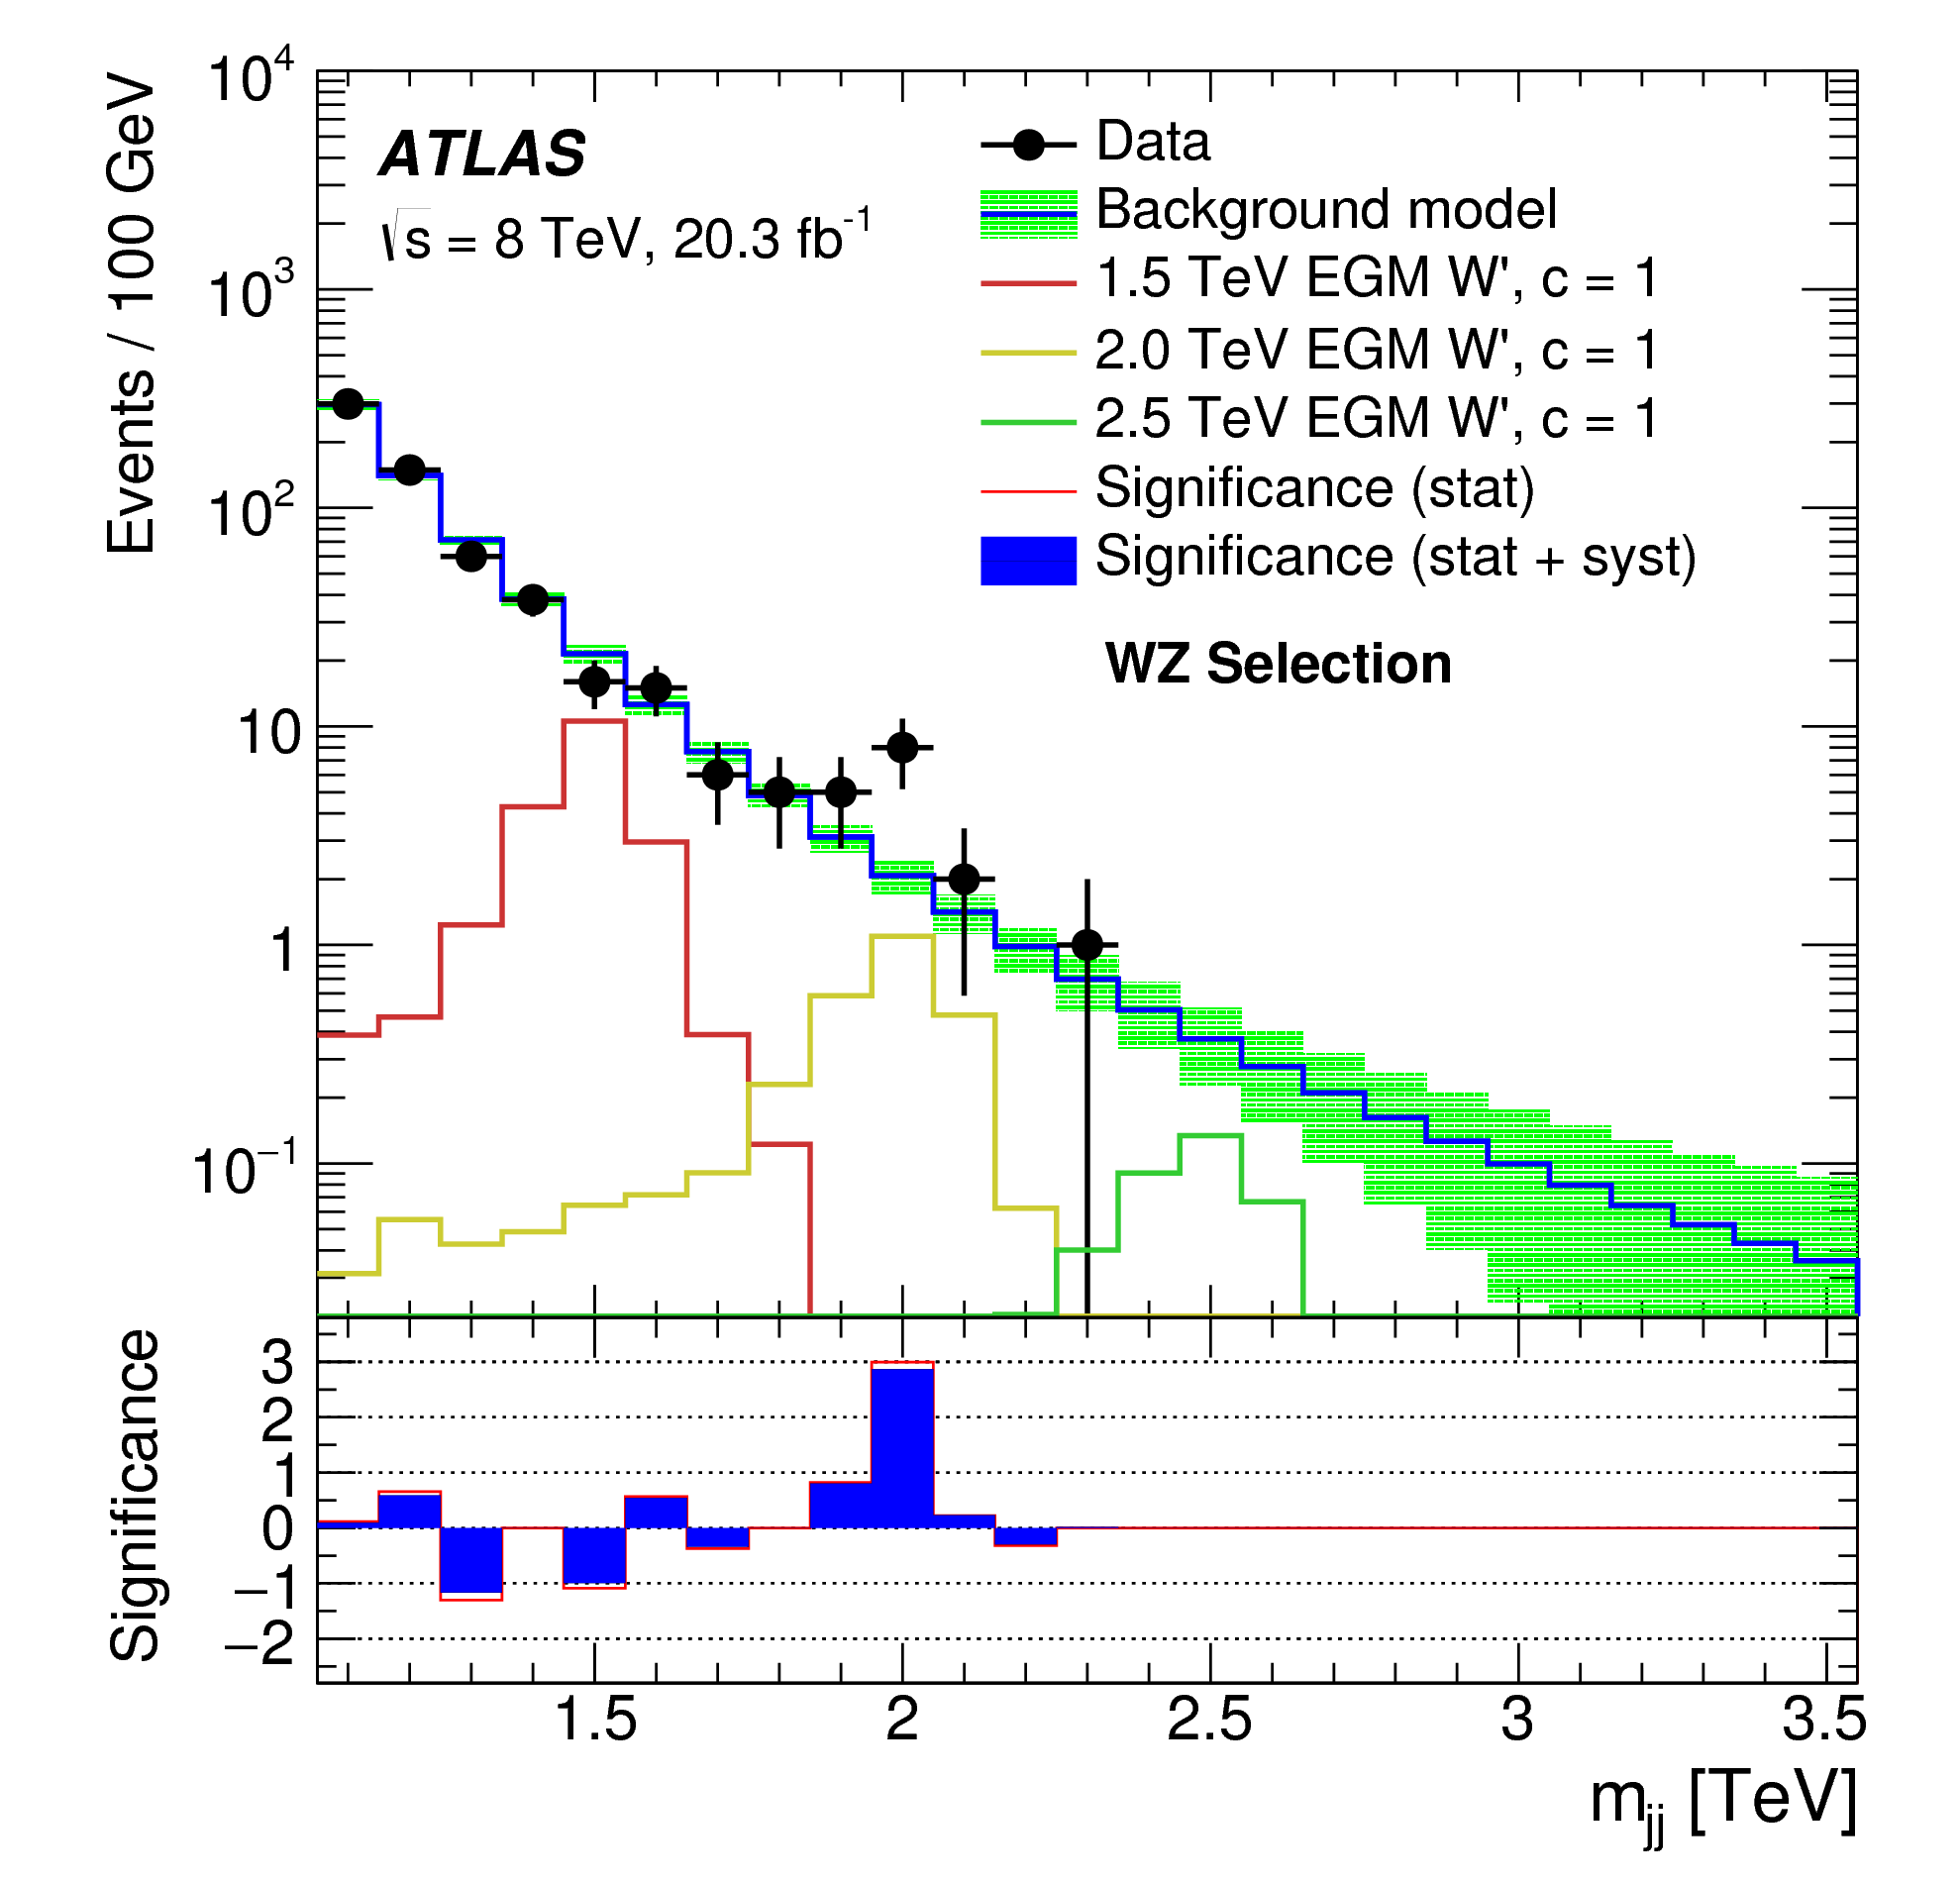
\includegraphics[height=0.3\textwidth]{figures/analysis/search1/misc/atlas_8tev.png}
    %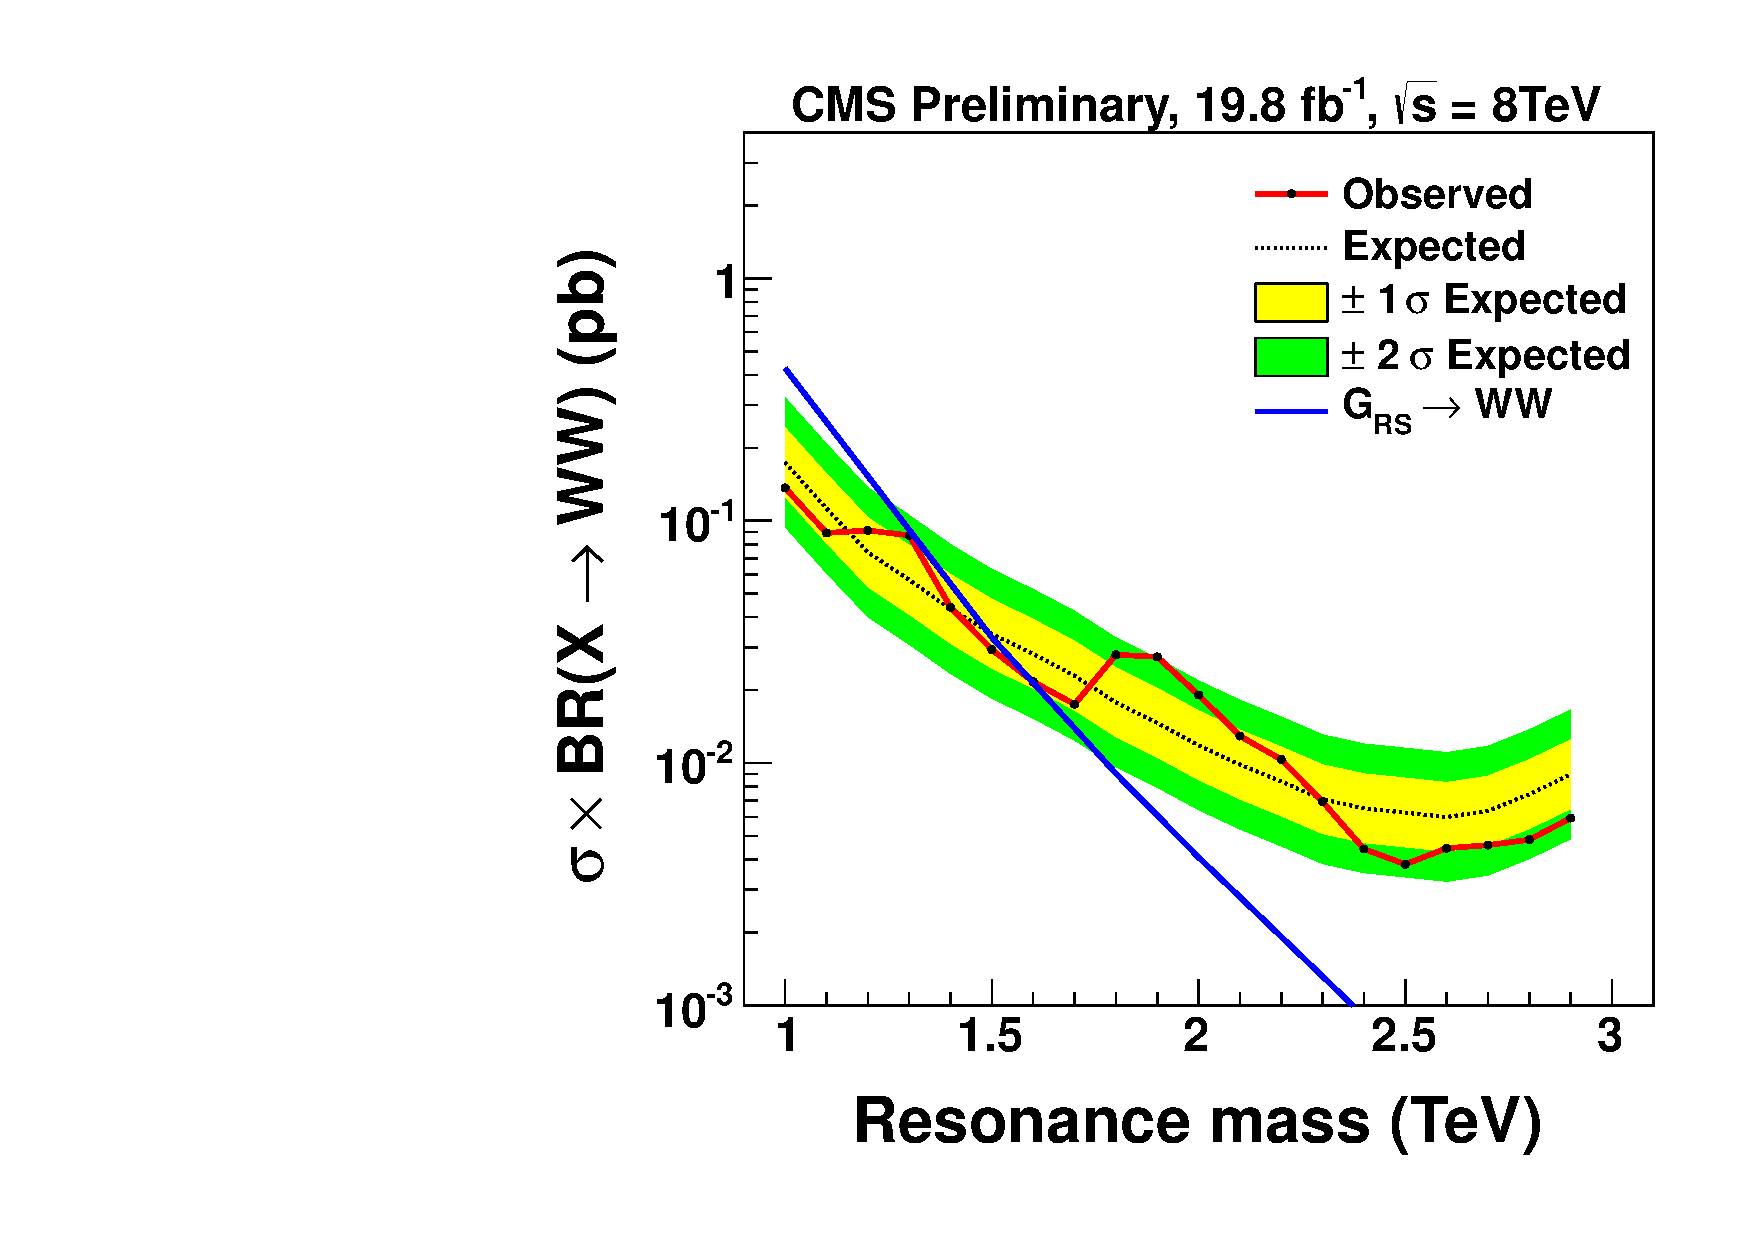
\includegraphics[height=0.3\textwidth]{figures/analysis/search1/misc/EXO-12-024_gWW.pdf}\\
    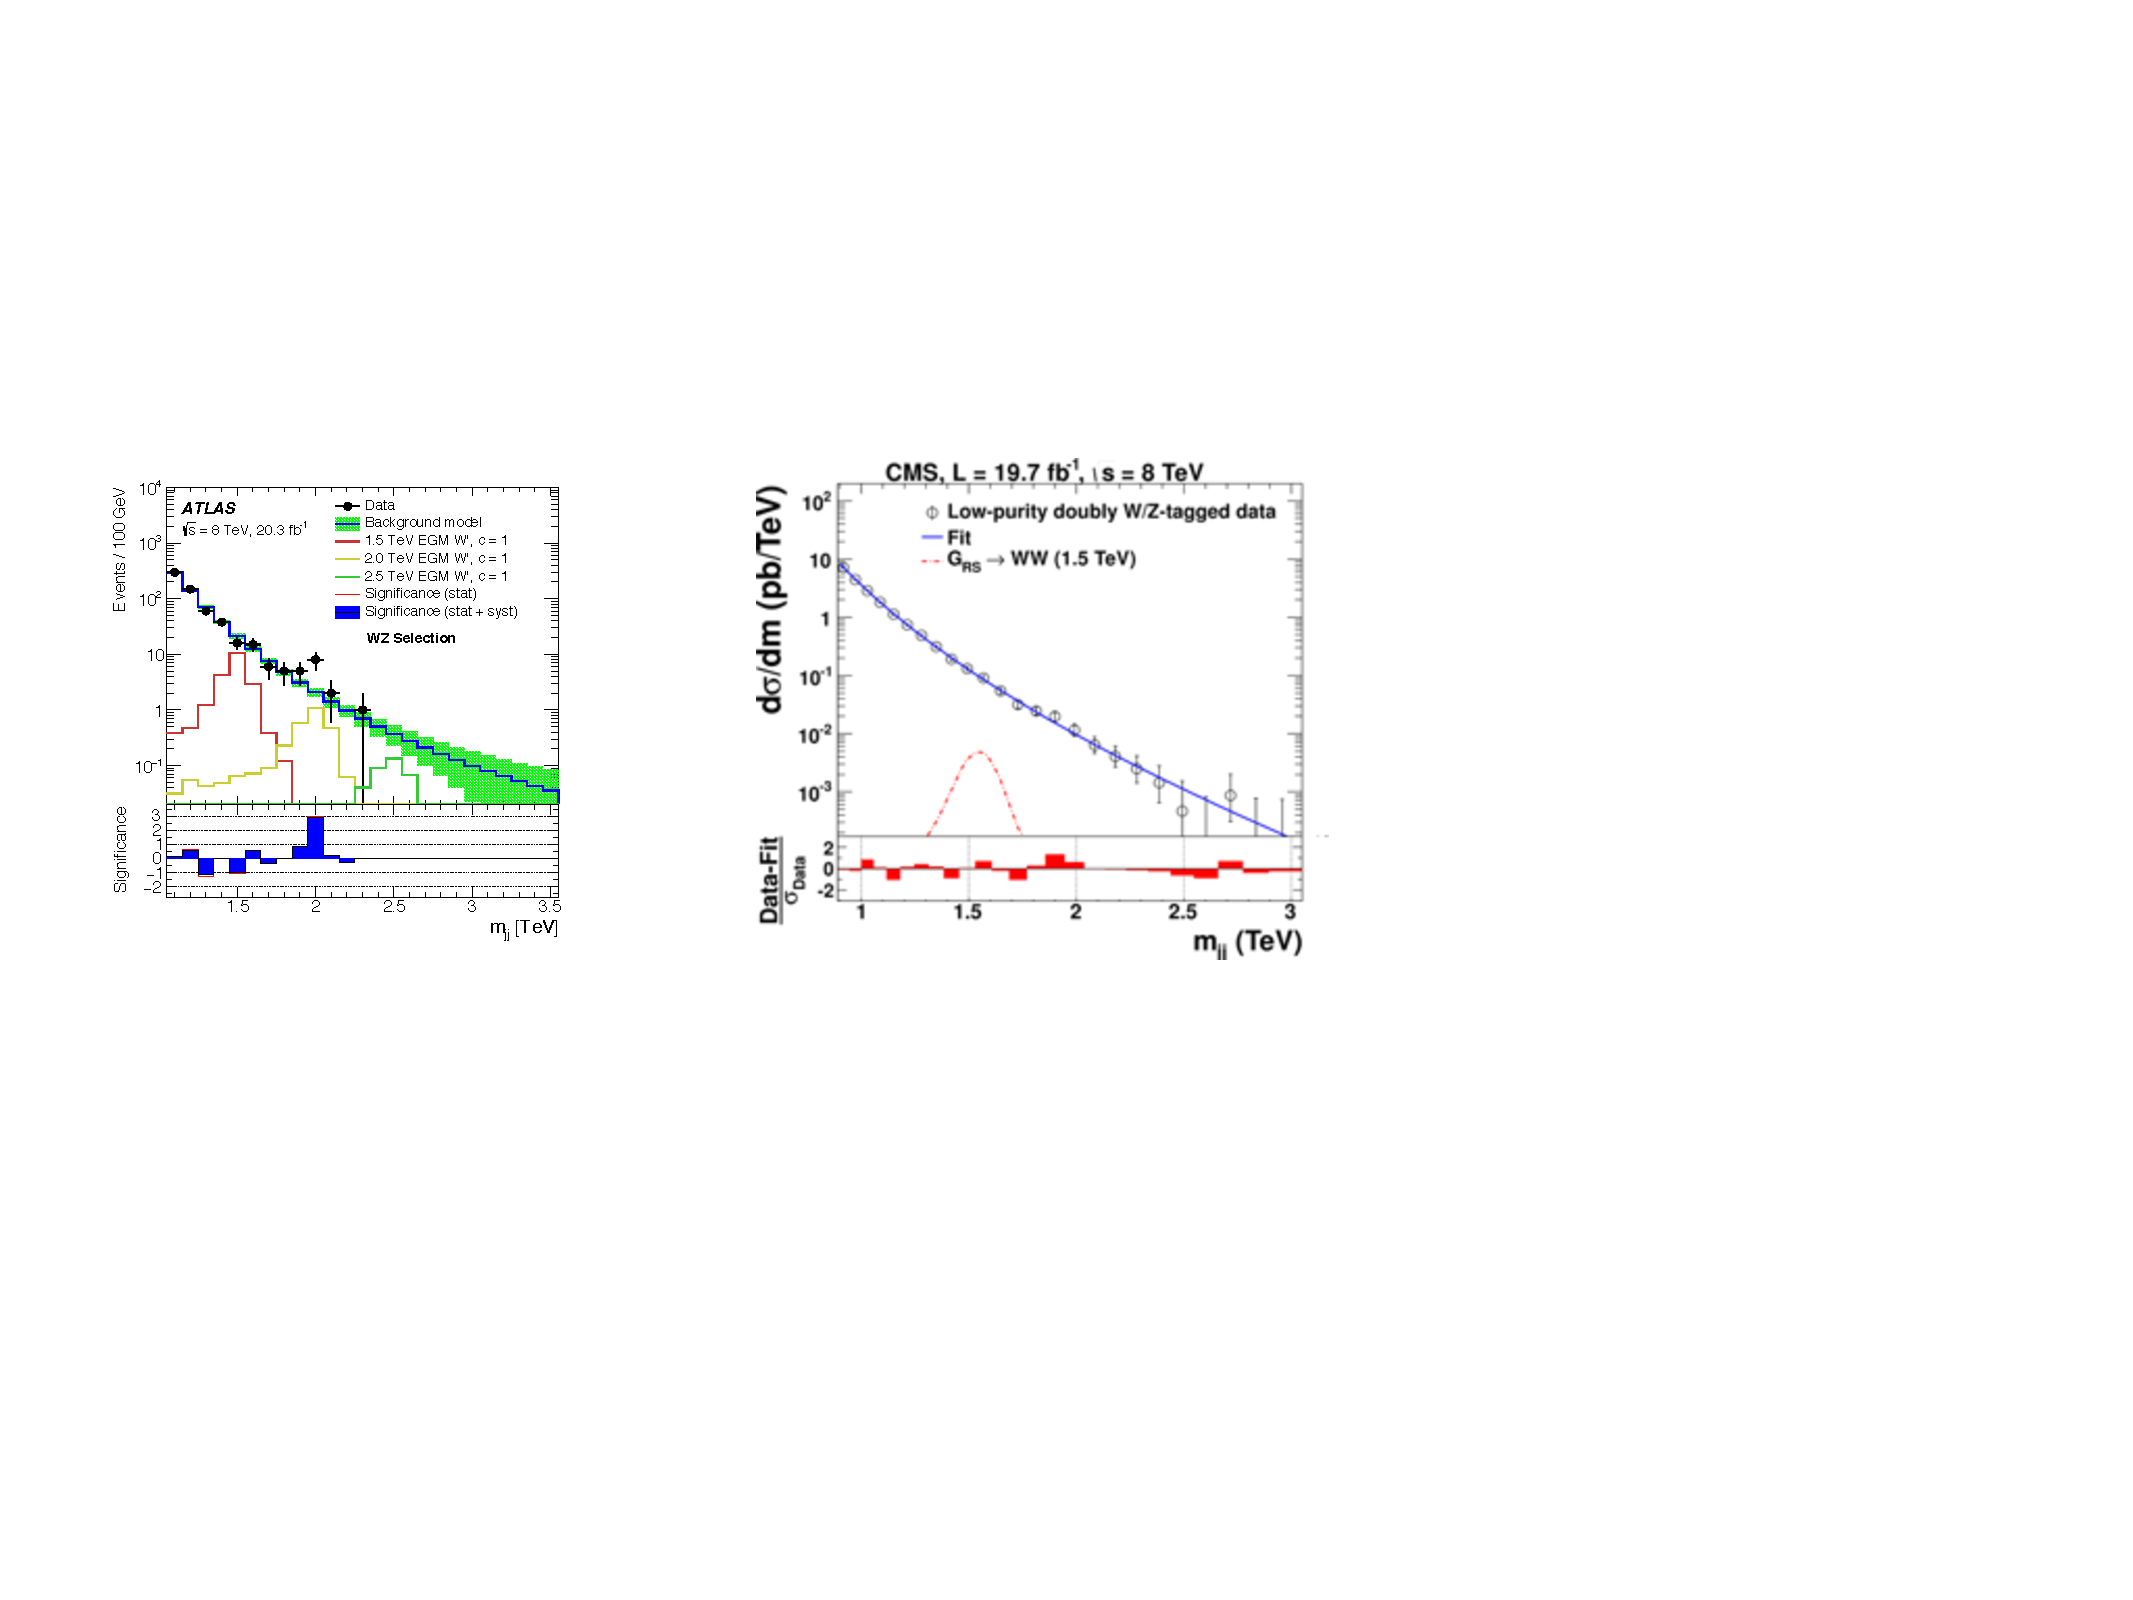
\includegraphics[height=0.2\textwidth]{figures/analysis/search3/misc/bumps2.pdf}\\
    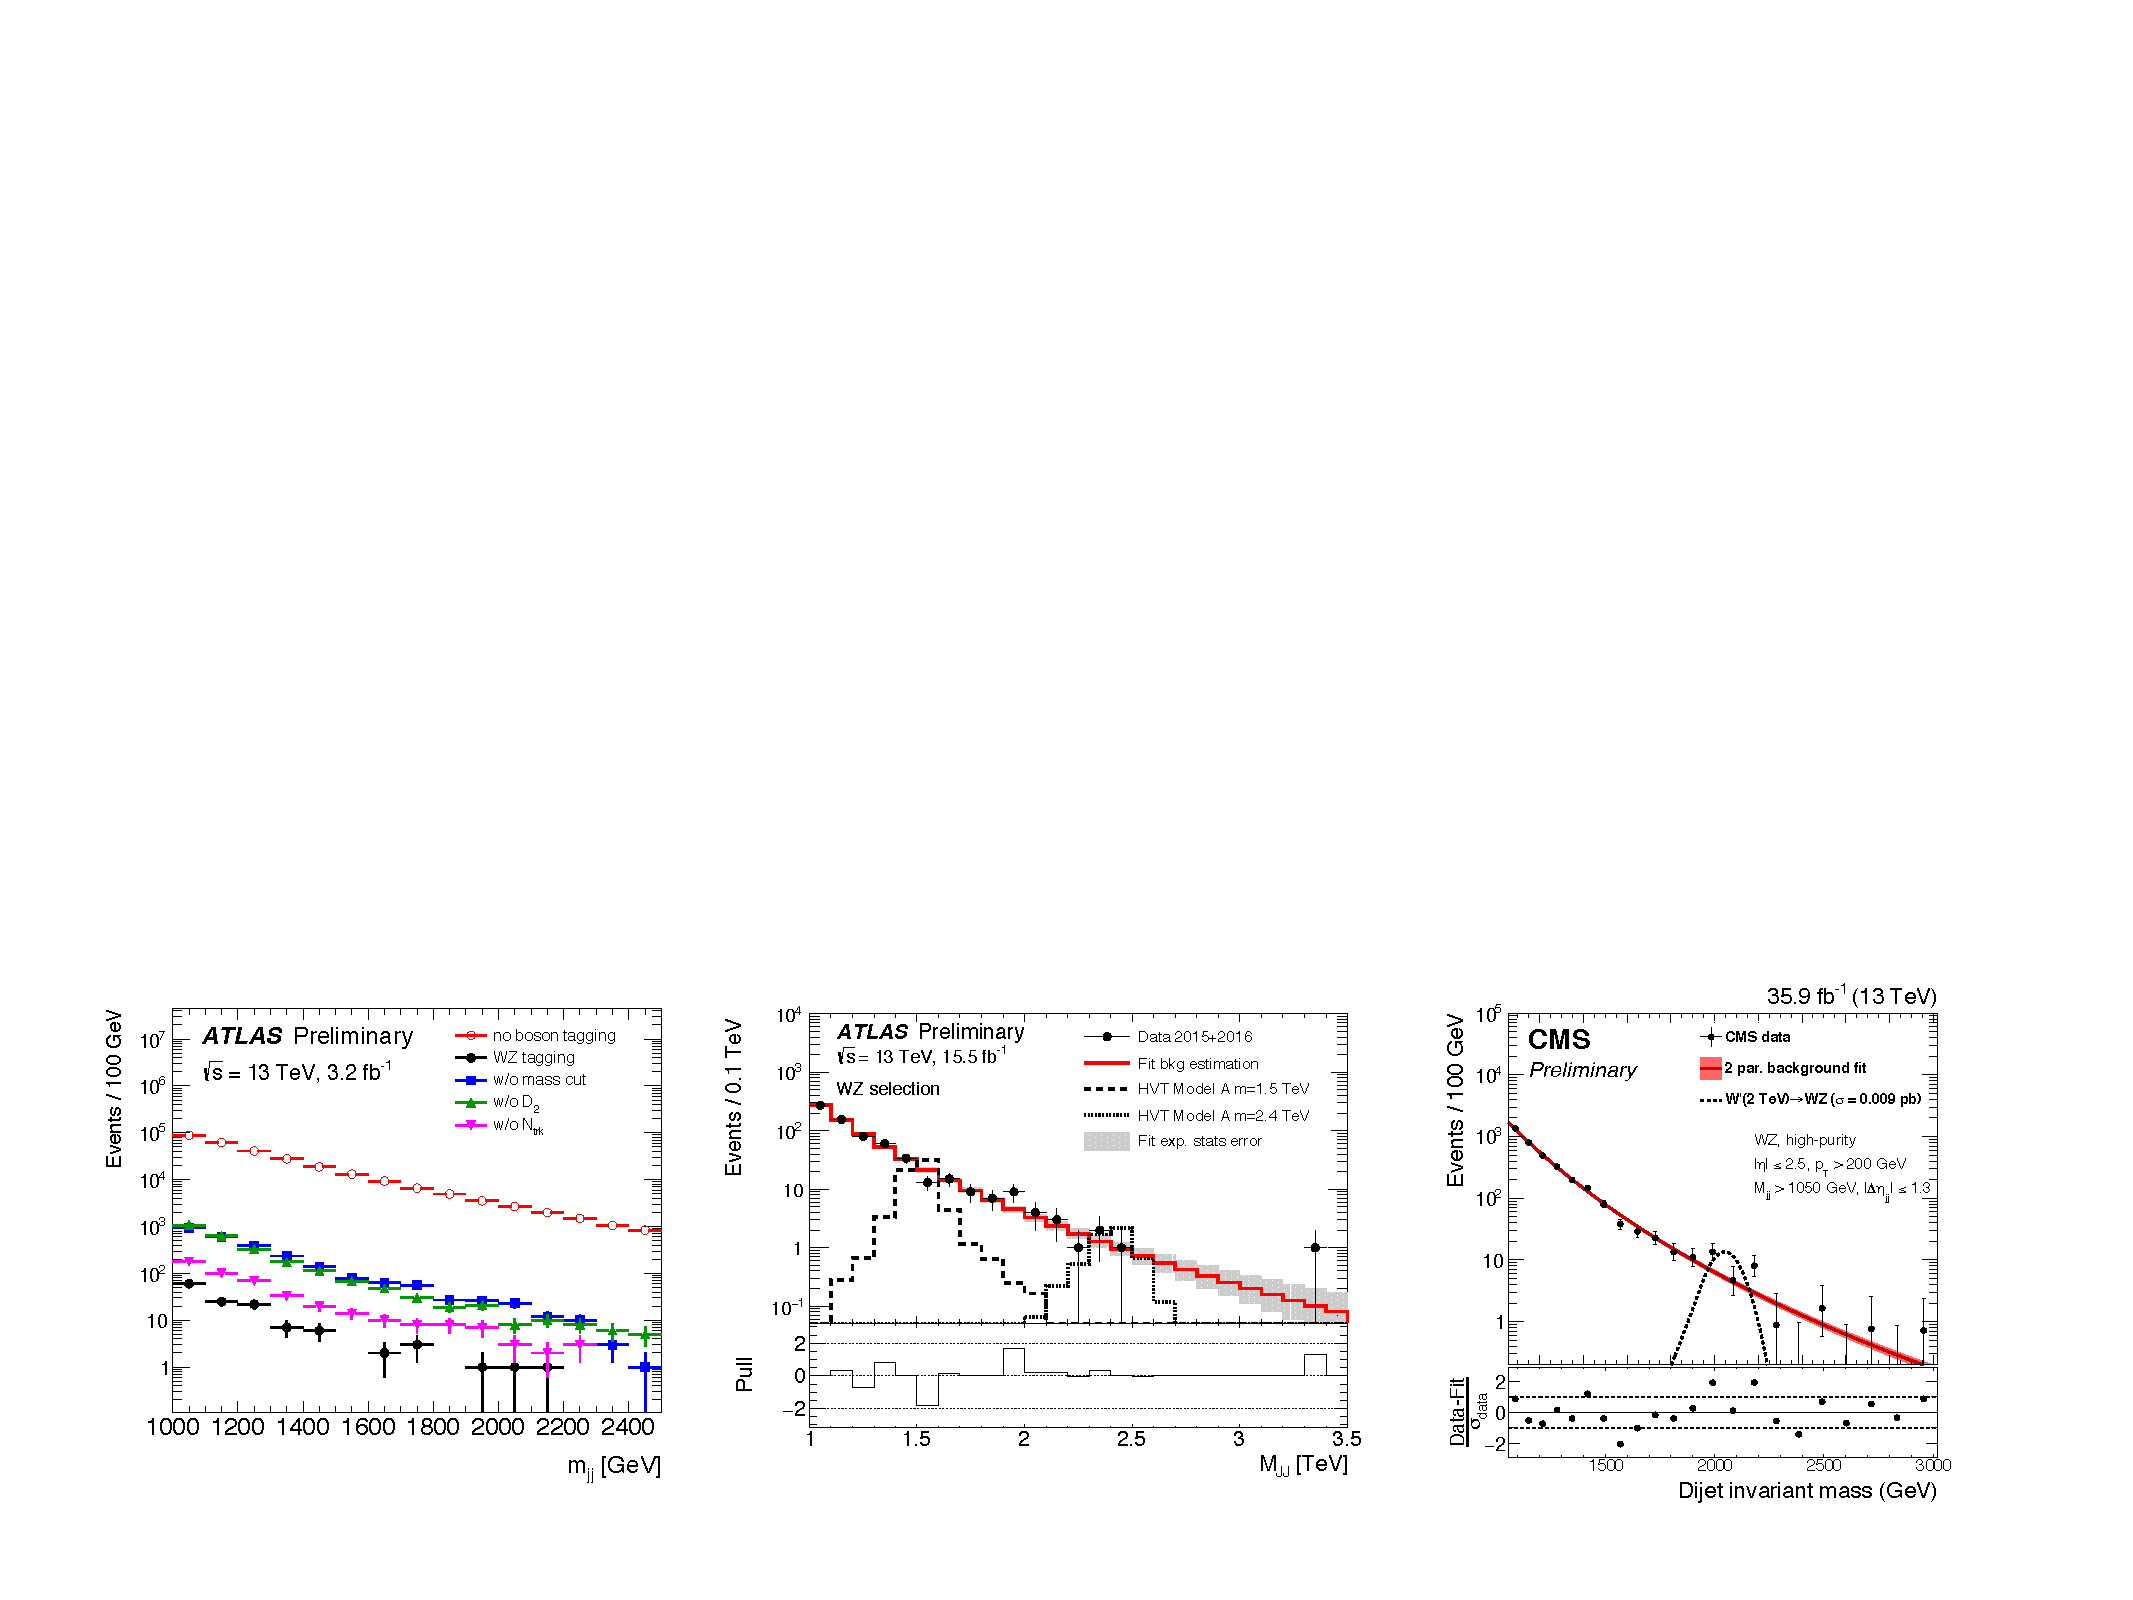
\includegraphics[height=0.2\textwidth]{figures/analysis/search3/misc/bumps1.pdf}\\
    \caption{Several small bumps observed in VV resonance searches in the all-hadronic final state, both in ATLAS and in CMS~\cite{stealth}.}
    \label{fig:searchIII:bumps}
\end{figure}
Due to their small size and the way the excesses seemed to slightly shift around, these were obviously not diboson resonances. However, could they be caused by us catching the tails of some non-SM boson with a mass slightly different from that of a SM vector boson, as illustrated in Figure~\ref{fig:searchIII:tails}?
\begin{figure}[ht] 
    \centering
    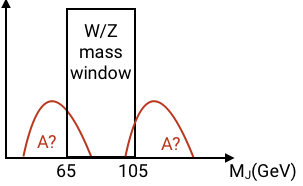
\includegraphics[width=0.3\textwidth]{figures/analysis/search3/misc/tails.png}
    \caption{Slight excesses in diboson analyses could be caused by catching the tail of a non-SM object peaking at slightly higher/lower jet mass than at the W/Z mass.}
    \label{fig:searchIII:tails}
\end{figure}
Further, these could be 4-pronged objects rather than 2-prong, which would cause the excess to vary in size depending on the 4-prong efficiency of the analysis specific W-tagger used.\newline
An explanation for the observed excesses was proposed in~\cite{Aguilar-Saavedra:2018xpl}. This paper pointed out that, if particles like \PWpr and \PZpr exist, an extended scalar sector is needed in order to give mass to the
vector bosons. These heavy scalars will decay to lighter bosons, if kinematically allowed, leading to multiboson signals from cascade decays. Some example signatures are illustrated in Figure~\ref{fig:searchIII:tribosons}.
\begin{figure}[ht] 
    \centering
    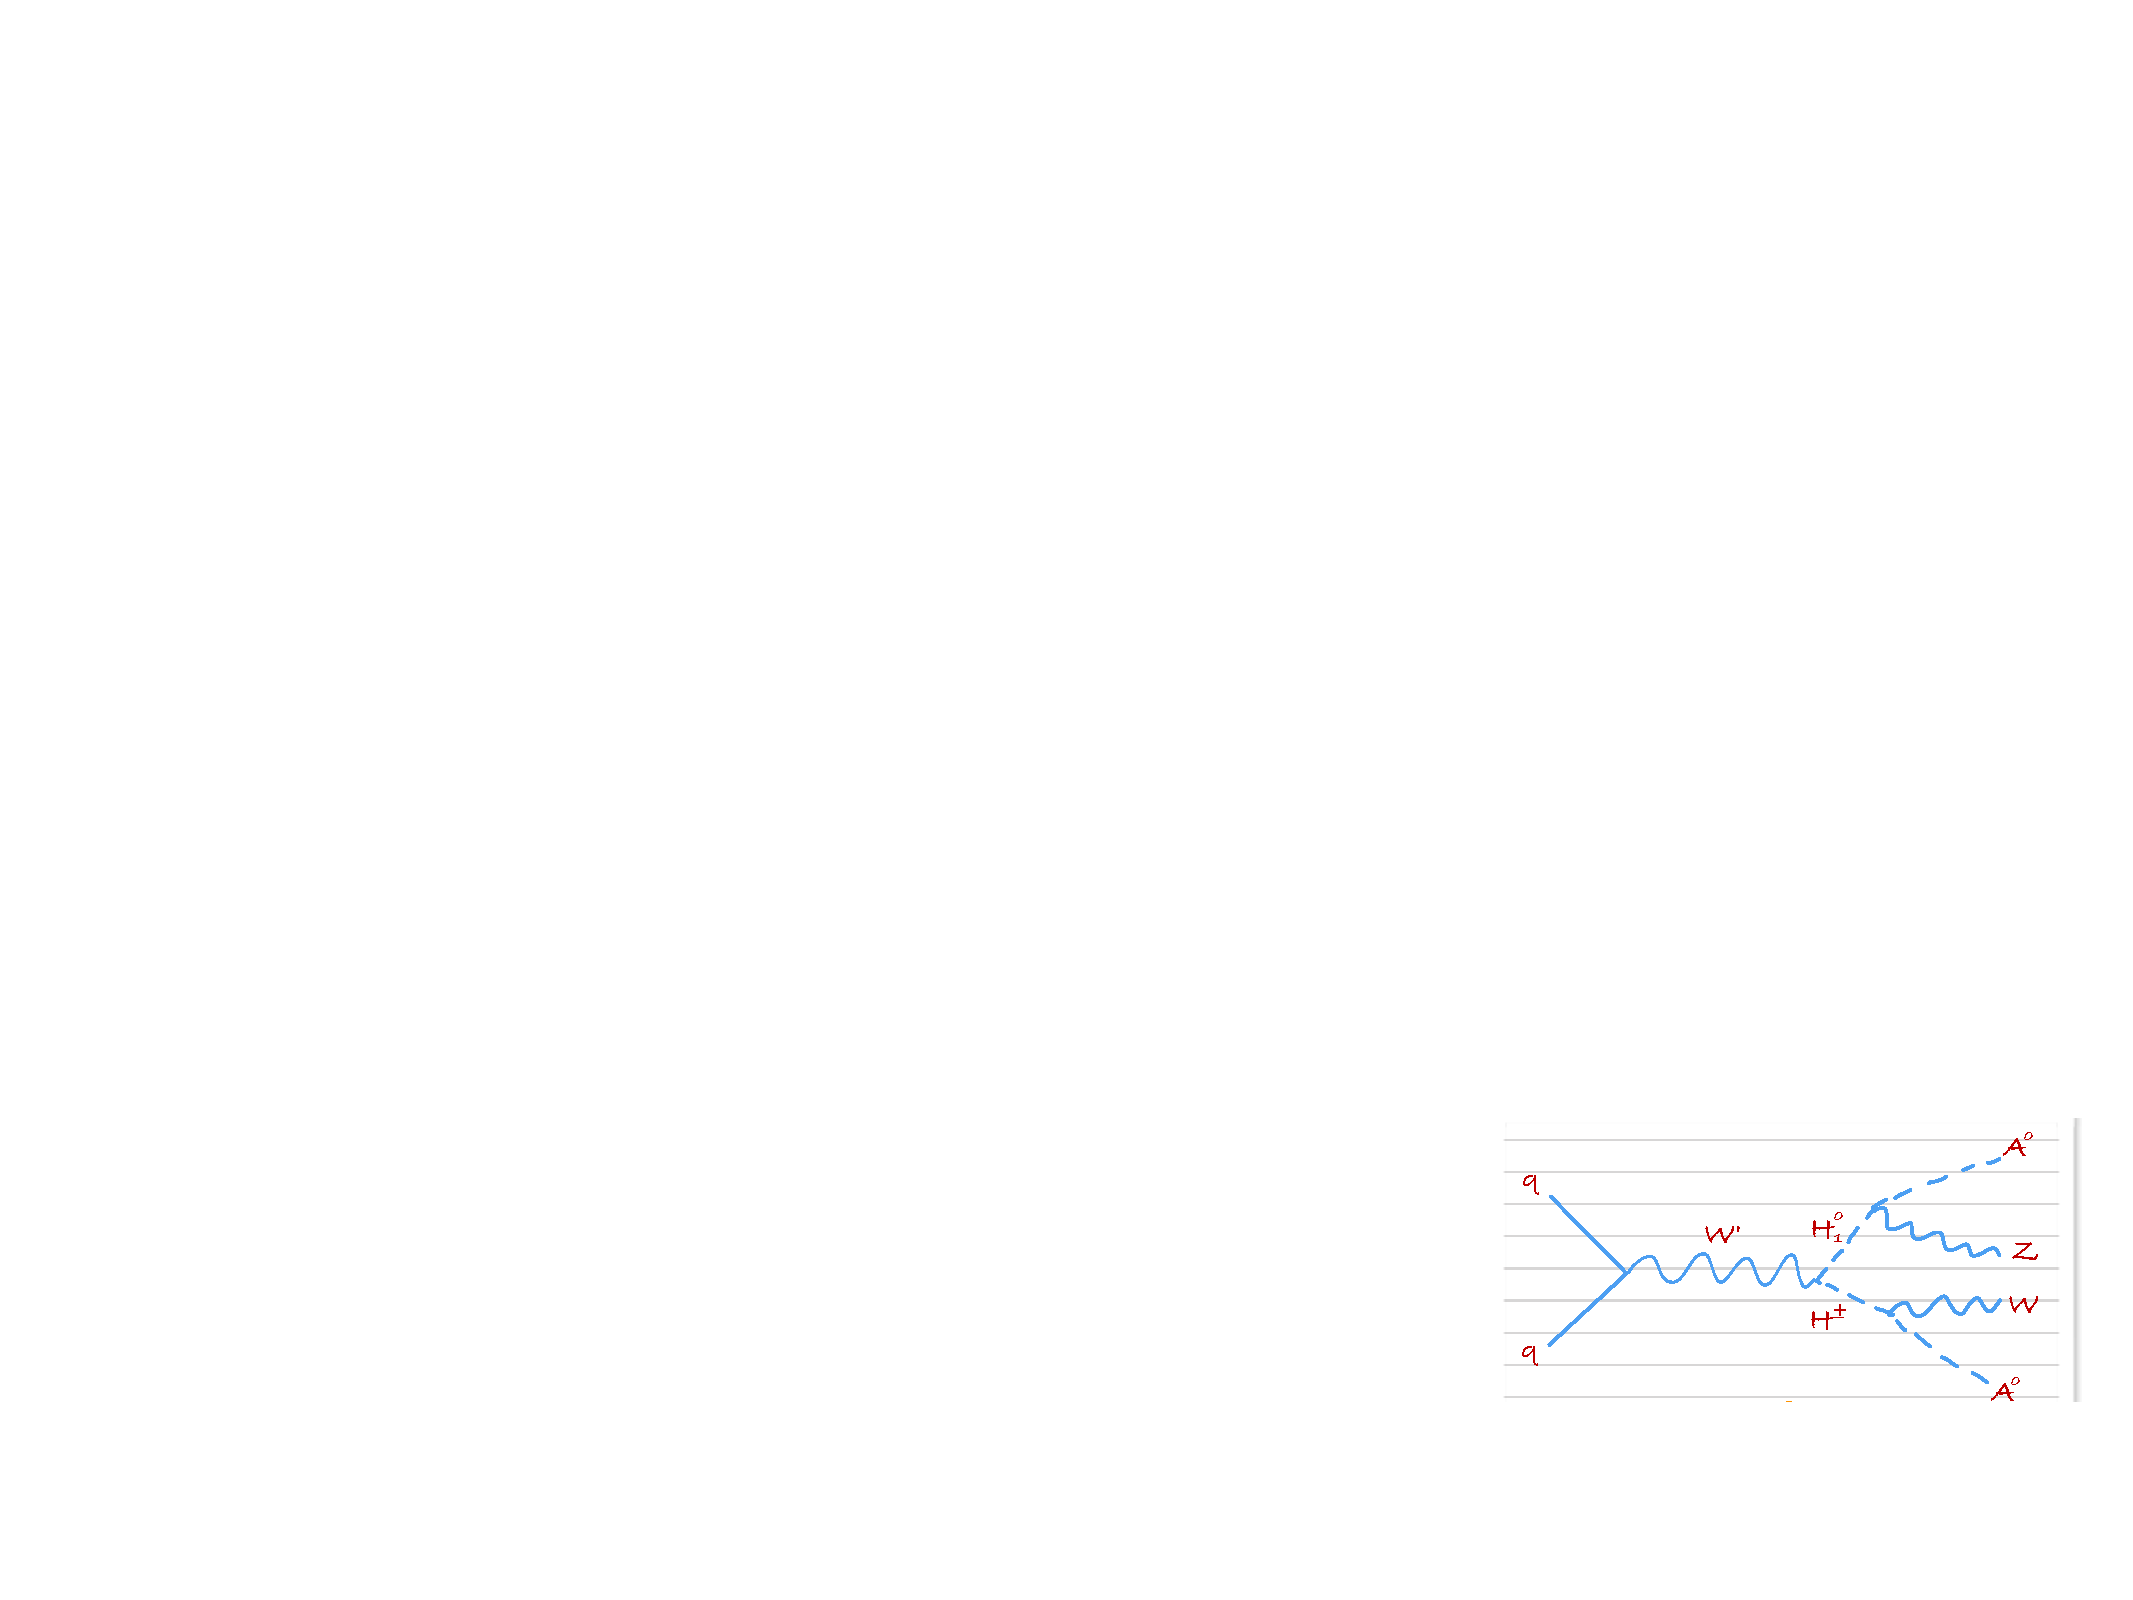
\includegraphics[height=2cm]{figures/analysis/search3/misc/quadri.pdf}
    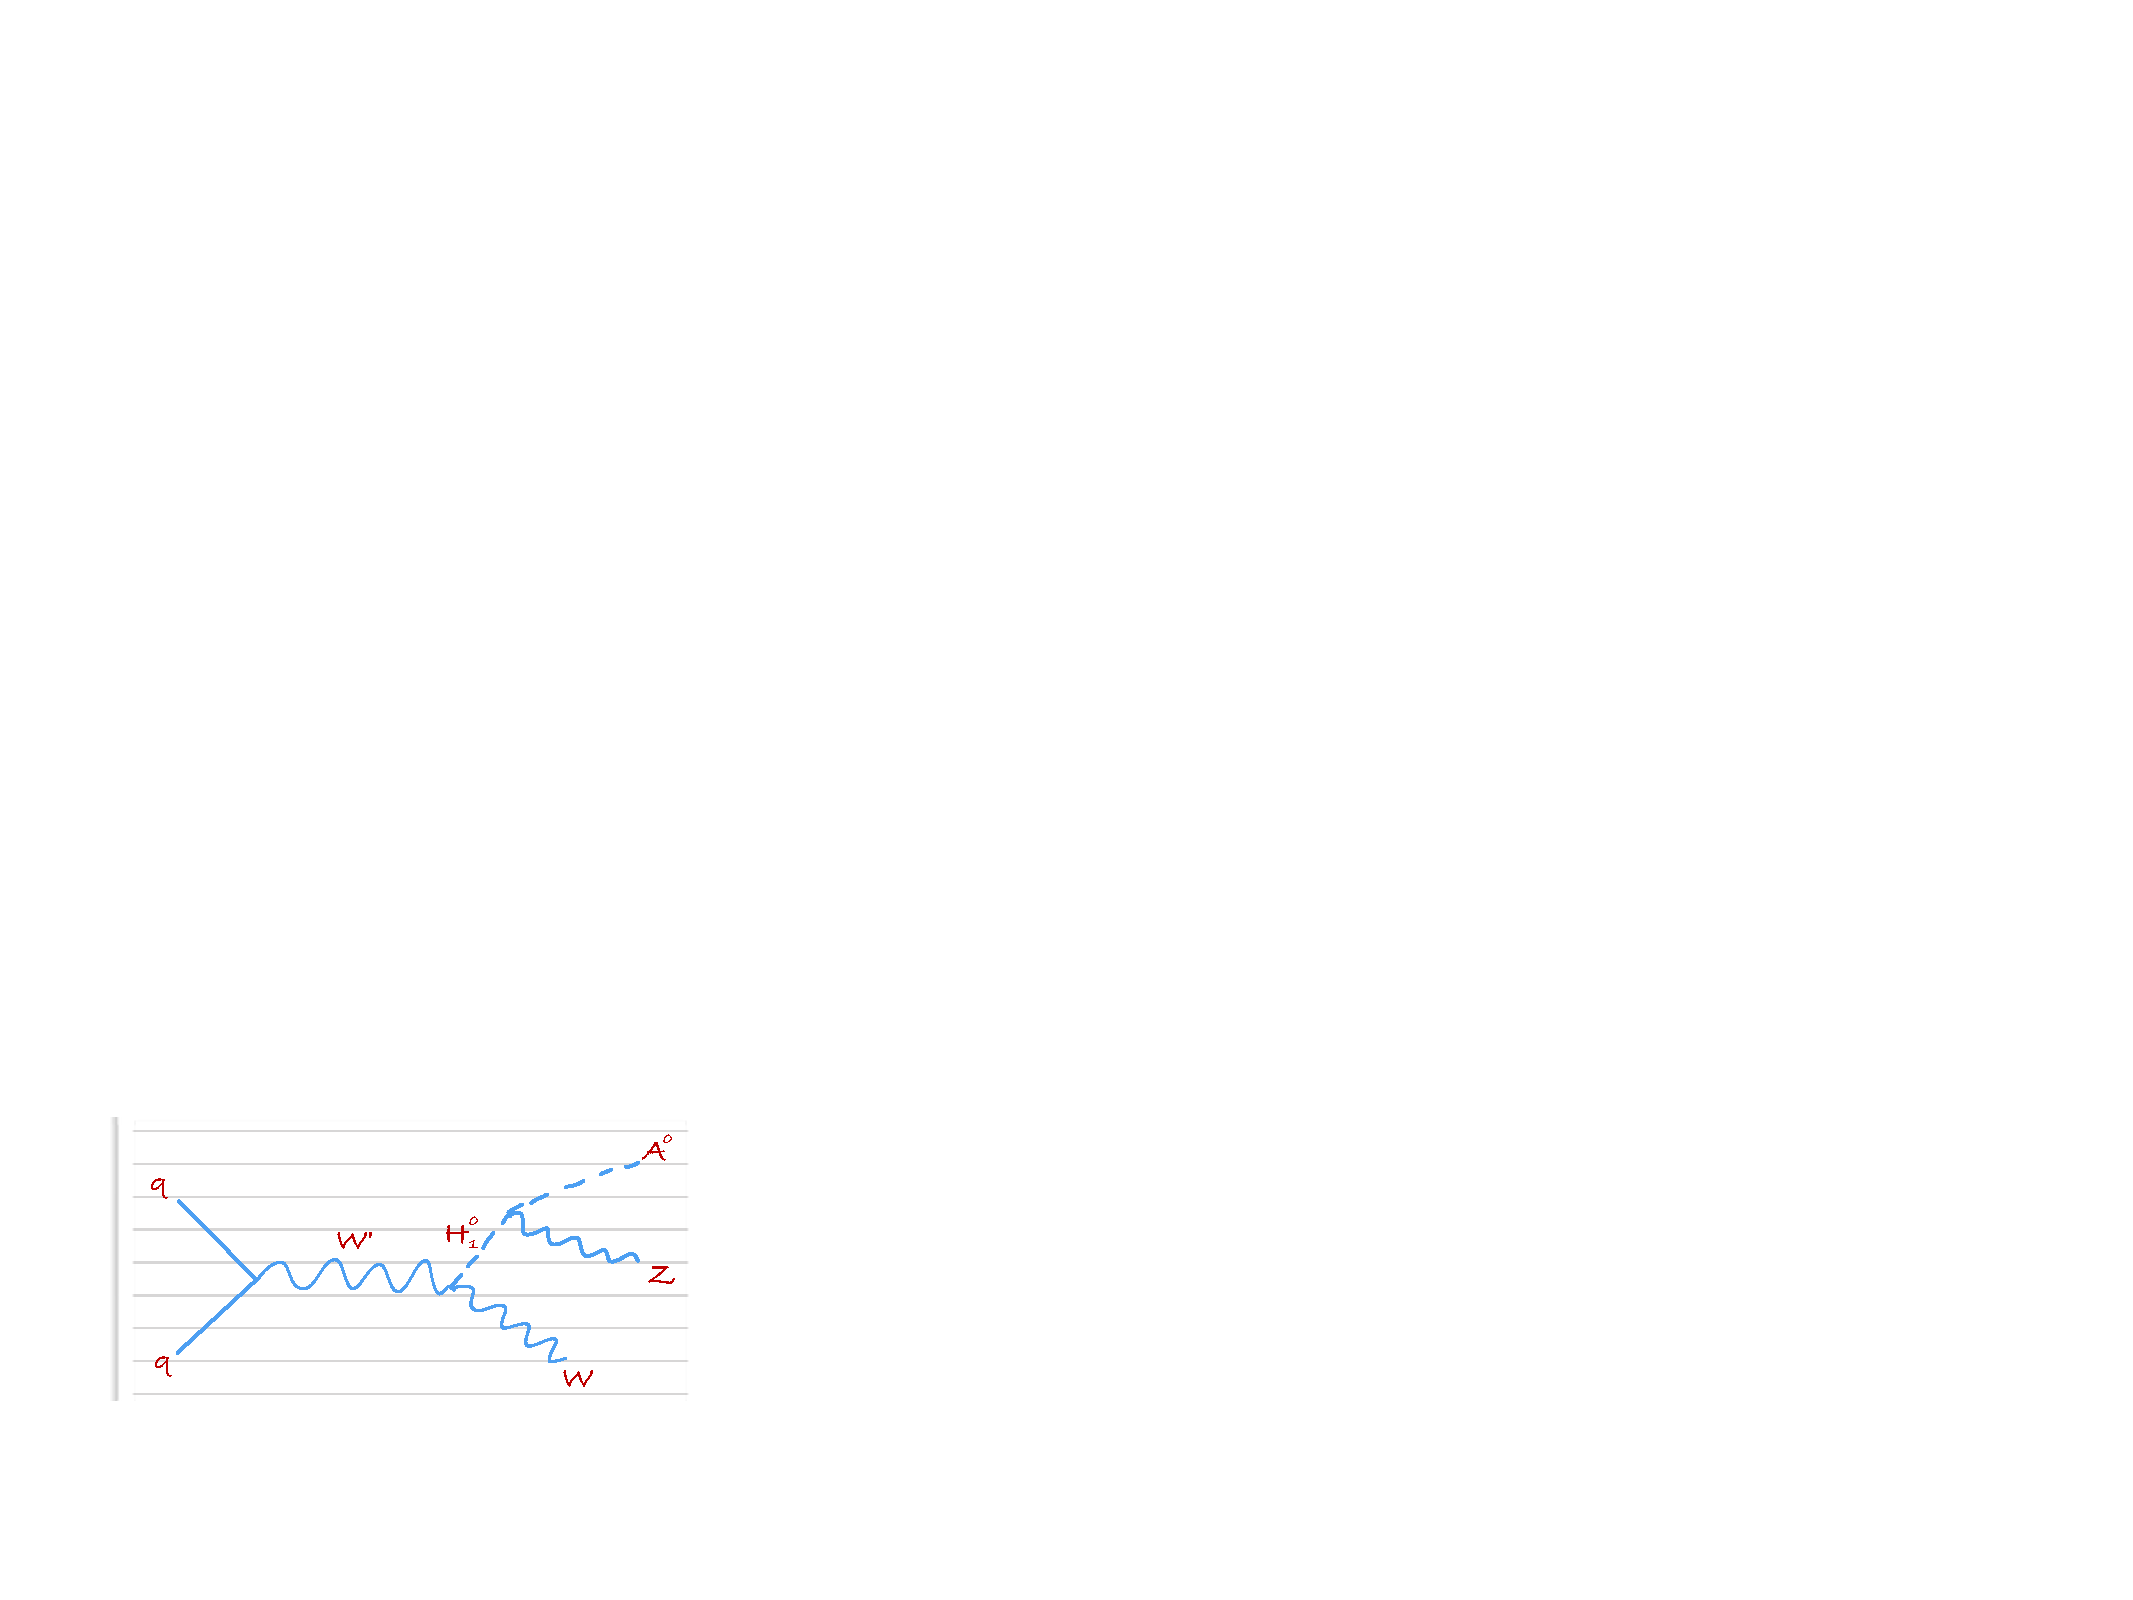
\includegraphics[height=2cm]{figures/analysis/search3/misc/tri1.pdf}
    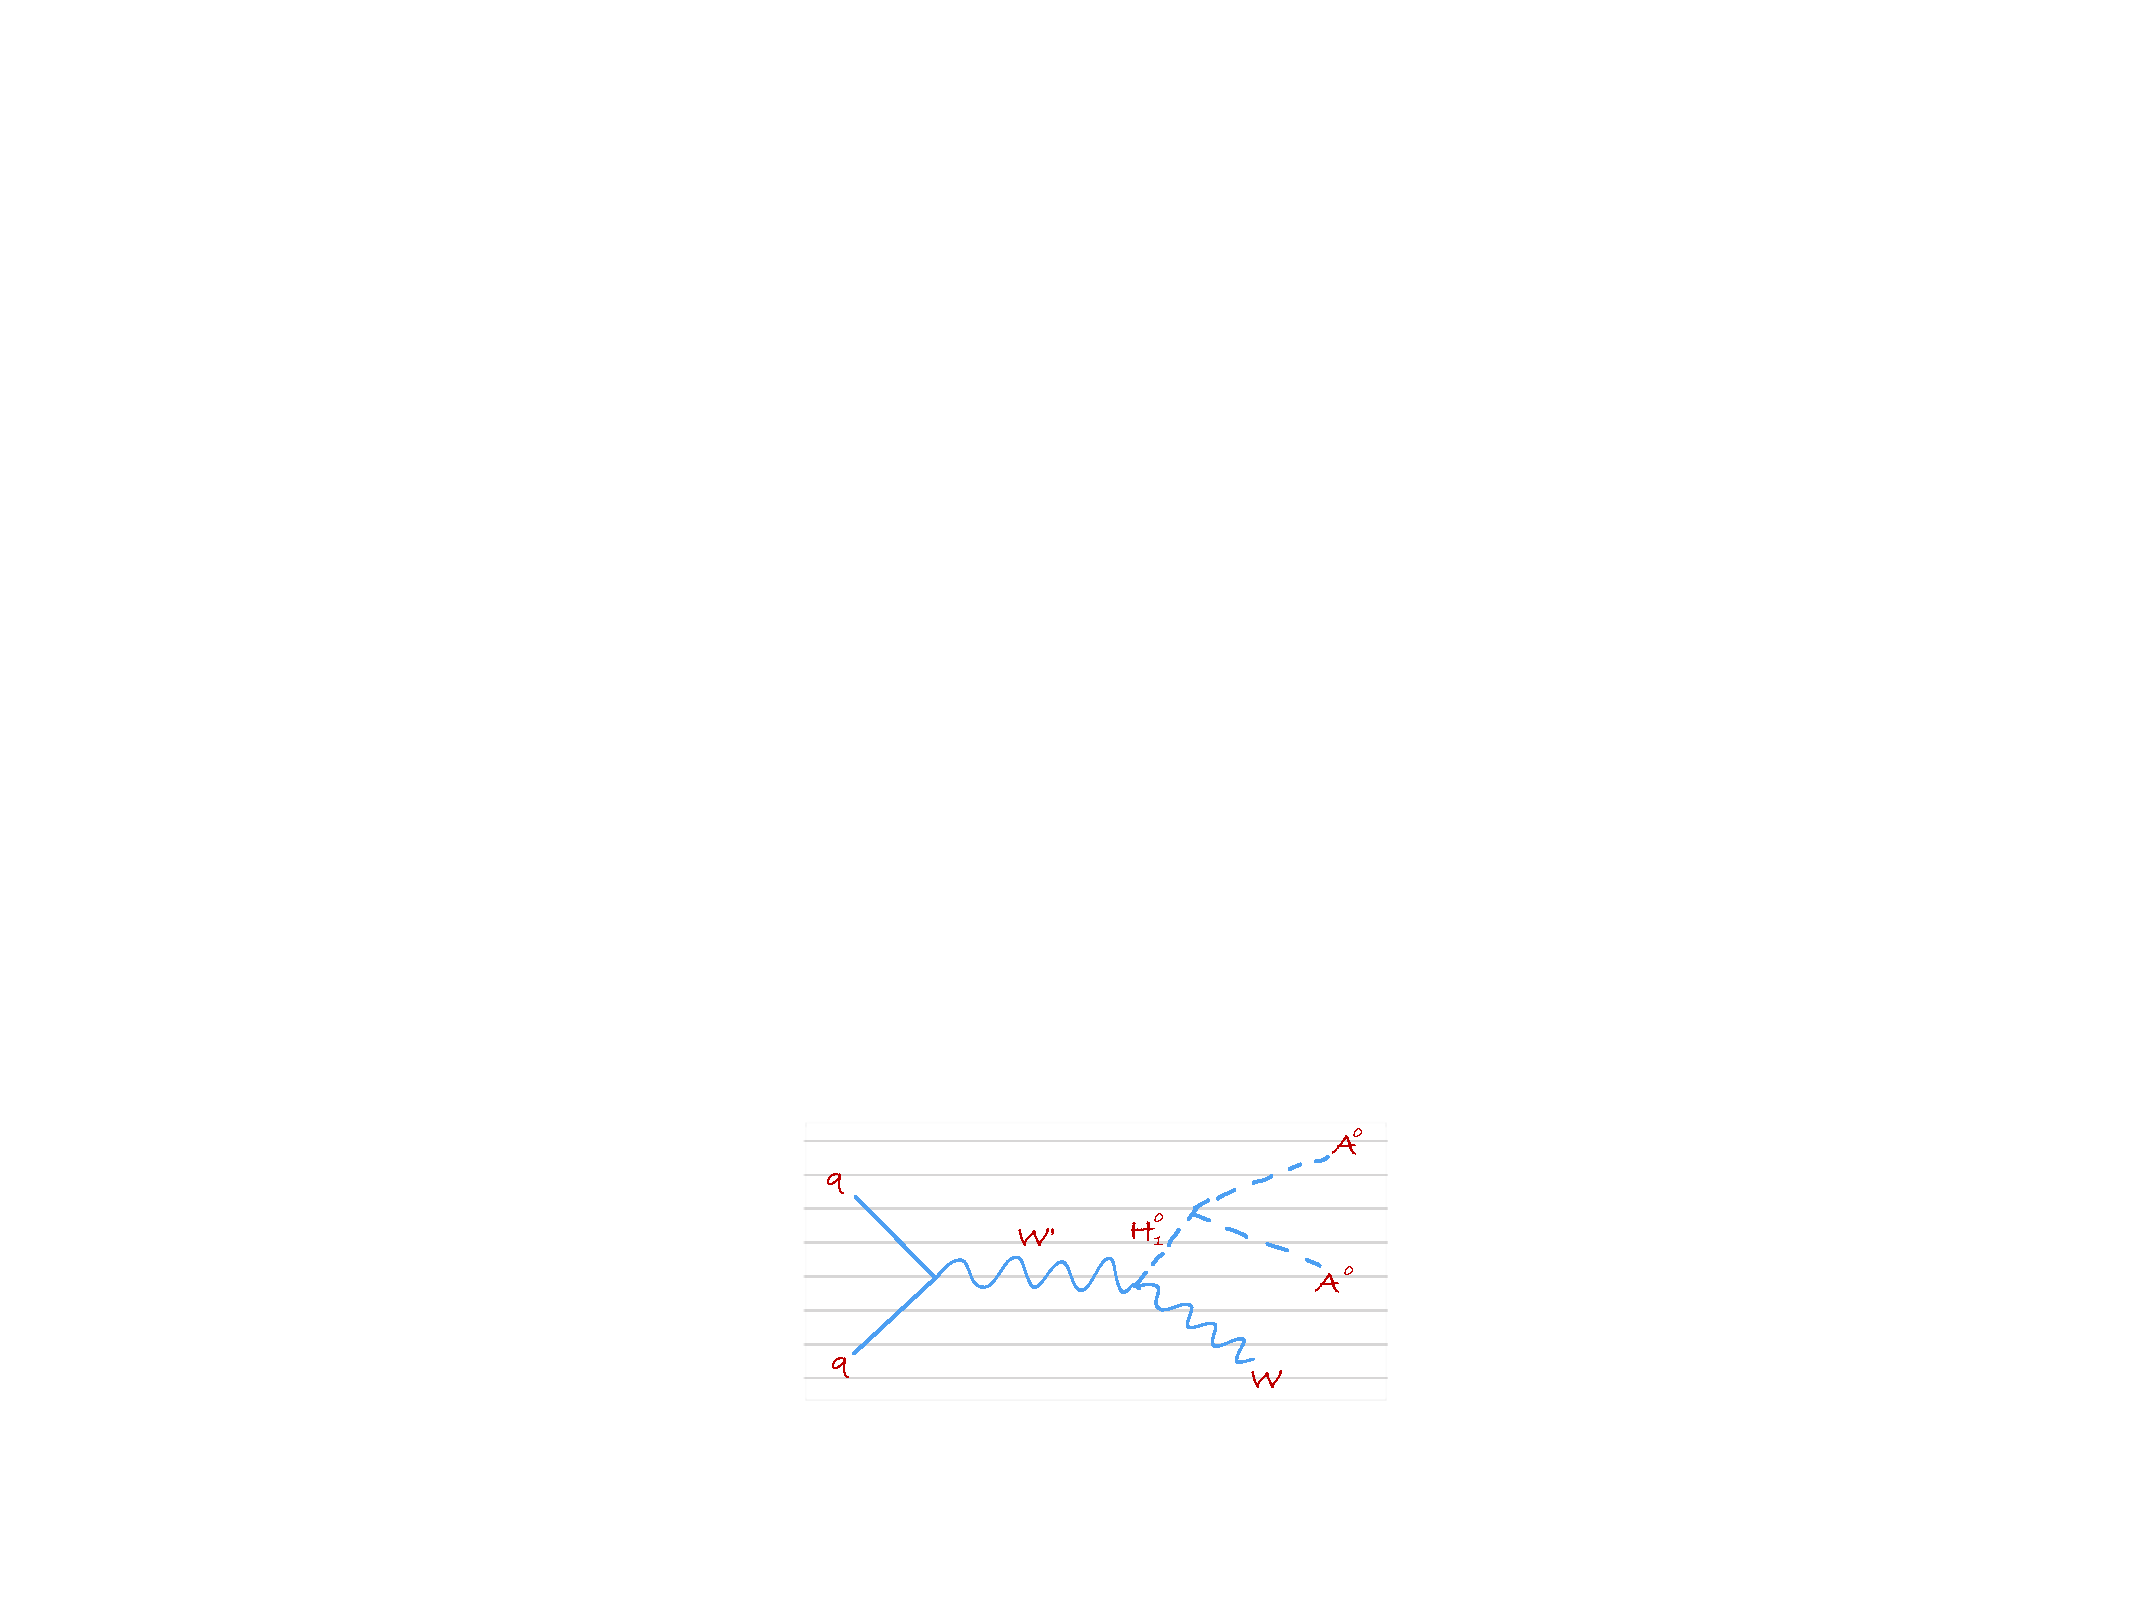
\includegraphics[height=2cm]{figures/analysis/search3/misc/tri2.pdf}
    \caption{A \PWpr decaying to a neutral $\rm{H}^0$ and a charged $\rm{H}^{\pm}$ scalar particle leading to a quadriboson final state (left), and a \PWpr decaying to a neutral scalar particle $\rm{H}^0$ and a \PW leading to a triboson final state (middle and right)~\cite{Aguilar-Saavedra:2018xpl}.}
    \label{fig:searchIII:tribosons}
\end{figure}
Signatures like these would peak in the groomed jet mass spectrum and, depending on what the final bosons decay into, have very different substructure profiles.\par
In order to effectively search for such types of signals, or any signal peaking in the softdrop jet mass spectrum, we therefore wanted to build a generic new framework allowing to look for peaks anywhere in the groomed mass - dijet invariant mass spectrum.
\subsection{Analysis strategy}
\subsection{Event selection}
\subsection{A mass and \PT decorrelated tagger}
\label{sec:searchIII:ddt}
\subsection{The multidimensional fit}